\documentclass[]{article}
\usepackage{lmodern}
\usepackage{amssymb,amsmath}
\usepackage{ifxetex,ifluatex}
\usepackage{fixltx2e} % provides \textsubscript
\ifnum 0\ifxetex 1\fi\ifluatex 1\fi=0 % if pdftex
  \usepackage[T1]{fontenc}
  \usepackage[utf8]{inputenc}
\else % if luatex or xelatex
  \ifxetex
    \usepackage{mathspec}
  \else
    \usepackage{fontspec}
  \fi
  \defaultfontfeatures{Ligatures=TeX,Scale=MatchLowercase}
\fi
% use upquote if available, for straight quotes in verbatim environments
\IfFileExists{upquote.sty}{\usepackage{upquote}}{}
% use microtype if available
\IfFileExists{microtype.sty}{%
\usepackage[]{microtype}
\UseMicrotypeSet[protrusion]{basicmath} % disable protrusion for tt fonts
}{}
\PassOptionsToPackage{hyphens}{url} % url is loaded by hyperref
\usepackage[unicode=true]{hyperref}
\hypersetup{
            pdfborder={0 0 0},
            breaklinks=true}
\urlstyle{same}  % don't use monospace font for urls
\usepackage[margin=1in]{geometry}
\usepackage{graphicx,grffile}
\makeatletter
\def\maxwidth{\ifdim\Gin@nat@width>\linewidth\linewidth\else\Gin@nat@width\fi}
\def\maxheight{\ifdim\Gin@nat@height>\textheight\textheight\else\Gin@nat@height\fi}
\makeatother
% Scale images if necessary, so that they will not overflow the page
% margins by default, and it is still possible to overwrite the defaults
% using explicit options in \includegraphics[width, height, ...]{}
\setkeys{Gin}{width=\maxwidth,height=\maxheight,keepaspectratio}
\IfFileExists{parskip.sty}{%
\usepackage{parskip}
}{% else
\setlength{\parindent}{0pt}
\setlength{\parskip}{6pt plus 2pt minus 1pt}
}
\setlength{\emergencystretch}{3em}  % prevent overfull lines
\providecommand{\tightlist}{%
  \setlength{\itemsep}{0pt}\setlength{\parskip}{0pt}}
\setcounter{secnumdepth}{0}
% Redefines (sub)paragraphs to behave more like sections
\ifx\paragraph\undefined\else
\let\oldparagraph\paragraph
\renewcommand{\paragraph}[1]{\oldparagraph{#1}\mbox{}}
\fi
\ifx\subparagraph\undefined\else
\let\oldsubparagraph\subparagraph
\renewcommand{\subparagraph}[1]{\oldsubparagraph{#1}\mbox{}}
\fi

% set default figure placement to htbp
\makeatletter
\def\fps@figure{htbp}
\makeatother

\usepackage{etoolbox}
\makeatletter
\providecommand{\subtitle}[1]{% add subtitle to \maketitle
  \apptocmd{\@title}{\par {\large #1 \par}}{}{}
}
\makeatother
\usepackage{setspace}\doublespacing
\usepackage{lineno}\linenumbers
% https://github.com/rstudio/rmarkdown/issues/337
\let\rmarkdownfootnote\footnote%
\def\footnote{\protect\rmarkdownfootnote}

% https://github.com/rstudio/rmarkdown/pull/252
\usepackage{titling}
\setlength{\droptitle}{-2em}

\pretitle{\vspace{\droptitle}\centering\huge}
\posttitle{\par}

\preauthor{\centering\large\emph}
\postauthor{\par}

\predate{\centering\large\emph}
\postdate{\par}

\date{}

\begin{document}

\section{Pagel's Lambda Estimates are Often
Inaccurate}\label{pagels-lambda-estimates-are-often-inaccurate}

\hfill\break

\textbf{Keywords}: Pagel's lambda, phylogenetic signal \hfill\break

\textbf{Short Title}: Inaccuracies in Pagel's Lambda \hfill\break

\section{Abstract}\label{abstract}

\{conclusion holds: interpreting the regression is not appreciably
different (in terms of slopes and f values)\}

\newpage

\section{Introduction}\label{introduction}

Investigating macroevolutionary patterns requires a phylogenetic
approach as species are non-independent by nature of their shared
ancestry. Since the first appropriate method was introduced by
Felsenstein (phylogenetic independent contrasts; (Felsenstein 1985)),
dozens of other methods have been developed and applied to increasingly
complex questions in macroevolutionary biology (e.g. (Grafen 1989);
(Harvey and Pagel 1991); (Rohlf 2001); ({\textbf{???}})). A particularly
useful measure in this field is phylogenetic signal, a quantification of
a trait's correspondence with the clade's phylogenic history.
Understanding the degree of phylogenetic signal present in a dataset is
paramount and identifies the mode with which a trait has evolved; high
measures of phylogenetic signal indicate a Brownian motion process,
whereas lower levels of phylogenetic signal indicate natural selection
or some other evolutionary force has influenced the traits evolutionary
history. \hfill\break

Several approaches to quantify phylogenetic signal exist. For continuous
data, the most common parameters used in the literature include Pagel's
lambda ({\textbf{???}}) and Blomberg's kappa ({\textbf{???}}). Pagel's
lambda has the advantage of being nested in the likelihood framework and
thus has also been utilized to simultaneously estimate and account for
phylogenetic signal while doing phylogenetic regressions or ANOVAs. At
the development of these estimation methods, clear recommendations on
the use and interpretation of this parameter were made based on data
simulations and error evaluations (Revell 2010). However, the accuracy
of the lambda estiamtion methods have not been fully evaluated, and
consequently many studies have substantially misused these methods.
\hfill\break

An earlier study ({\textbf{???}}), breifly addressed this topic by
showing how uninformative smaller phylogenies are when estimating
various evolutionary parameters, such as Pagel's lambda. However, it
remains unknown the degree to which lambda estimates accurately
represent degree of phylogenetic signal, and thus we fully explicate the
extent to which Pagel's lambda estimation methods can and have been
misused in recent macroevolutionary studies. Here we take a
comprehensive approach to demonstrate the scenarios under which
estimated Pagel's lambdas accurately reflect known lambdas. We then
demonstrate the effect of these, at times, dubious estimation methods on
significance testing when used in a pgls framework. Finally, we perform
a meta-analysis of research published in 2019 employing Pagel's lambda
estimation methods to demonstrate the uses and misuses of this method in
the literature. This investigation provides evidence for the
circumstances under which estimating Pagel's lambda can be informative,
and which interpretations or uses are misleading with the hope of moving
the field towards more appropriate employment of our methodological
toolbox.

\section{Methods and Results}\label{methods-and-results}

\subsection{\texorpdfstring{\emph{Simulated
trait}}{Simulated trait}}\label{simulated-trait}

To assess the accuracy of Pagel's lambda estimations, we simulated
pure-birth phylogenies of increasing size, ranging in tip number from 32
to 1028. We then scaled the phylogenies by known lambda values ranging
from 0 to 1 (0.05 intervals; 50 trees per lambda value per tree size)
and generated trait data by simulating a single continuous variable on
each scaled phylogeny under Brownian motion. With the generated
datasets, we used phylogenetic generalized least squares (PGLS) to
estimate lambda values and extracted the model fit likelihood values.
Finally, we calculated model fit likelihood values of PGLS models using
the known lambdas as the input lambdas in the model and using ordinary
least squares models (OLS; lambda = 0). \hfill\break

To visualize the accuracy of the lambda estimation methods, we first
plotted known lambdas (input lambdas) against the estimated lambdas. We
also calculated rates of model misspecification for each phylogeny size,
quantifying the rate at which models with known lambdas of 0 incorrectly
define a significant phylogenetic signal as well as the rate at which
models with known lambdas \textgreater{} 0 incorrectly estimate lambda
as not significantly different from 0. \hfill\break

Results from these data (Figure 1).

\subsection{\texorpdfstring{\emph{Simulated ANOVA and
Regressions}}{Simulated ANOVA and Regressions}}\label{simulated-anova-and-regressions}

To ascertain the statistical performance of PGLS lambda estimation
methods, we generated datasets with two trait variables across a range
of known lambda values and correlation strengths. First, the independent
variable (both continuous and binary) was generated in the same manner
as the simulation procedures above. For each independent variable, we
then generated a continuous dependent variable with input slopes ranging
from 0 to 1 (0.25 intervals). From these data, used PGLS to estimate
slope as well as F-values to assess the accuracy and error rates of
these regression and ANOVA analyses while estimating lambdas. Finally,
we again fit the dependent variable to the independent variable,
estimated the slope and F-values using PGLS with the known lambdas as
the input lambdas as well as under OLS. \hfill\break

We calculated error rates \ldots{} \hfill\break

Scaling and trait generation procedures for both simulation methods was
repeated with symmetrical and ladder phylogeny shapes. Results of these
phylogeny shapes were consistent with pure-birth phylogeny results and
can be found in the Supplemental Materials. All analyses were performed
in R v3.6.0 ({\textbf{???}}) using the packages \texttt{geiger}
({\textbf{???}}) and \texttt{caper} ({\textbf{???}}), and the
corresponding scripts can be found in the Supplemental Materials.
\hfill\break

Results from these data (Figure 2).

\subsection{\texorpdfstring{\emph{Meta-Analysis of Empirical
Results}}{Meta-Analysis of Empirical Results}}\label{meta-analysis-of-empirical-results}

Despite the urging of Boettiger and colleagues to publish confidence
intervals with all lambda parameter estimates, only 18\% of papers
published in 2019 do so. \hfill\break

More methods paragraphs \hfill\break

Results from these dta (Figure 3).

\section{Discussion}\label{discussion}

Using the estimated lambda values from pgls are not useful. The
questions of whether or not signal exists is appropriate, but inferring
more from lambda \emph{magnitude} is inappropriate. \hfill\break

More discussion paragraphs

\newpage

\section{References}\label{references}

\setlength{\parindent}{-0.25in} \setlength{\leftskip}{0.25in}
\setlength{\parskip}{8pt} \noindent

\hypertarget{refs}{}
\hypertarget{ref-Felsenstein1985}{}
Felsenstein, J. 1985. Phylogenies and the comparative method. American
Naturalist 125:1--15.

\hypertarget{ref-Grafen1989}{}
Grafen, A. 1989. The phylogenetic regression. Philosophical Transactions
of the Royal Society of London B, Biological Sciences 326:119--157.

\hypertarget{ref-HarveyPagel1991}{}
Harvey, P. H., and M. D. Pagel. 1991. The comparative method in
evolutionary biology. Oxford University Press, Oxford.

\hypertarget{ref-Revell2010}{}
Revell, L. J. 2010. Phylogenetic signal and linear regression on species
data. Methods in Ecology and Evolution 1:319--329.

\hypertarget{ref-Rohlf2001}{}
Rohlf, F. J. 2001. Comparative methods for the analysis of continuous
variables: Geometric interpretations. Evolution 55:2143--2160.

\newpage

\section{Figure Legends}\label{figure-legends}

\textbf{Figure 1}. Accuracy of Pagel's lambda estimations across known
lambda inputs on various tree sizes. As trees increase in size, the
estimates more closely resemble the input lambdas, however considerable
and concerning variation is apparent in trees smaller than those with
256 tips.

\textbf{Figure 2}. Estimated ANOVA slopes under PGLS. Across tree sizes,
the mean estimated slope matches the input slope, and as trees increase
in size, the variance around this mean estimate decreases. However, for
trees with fewer than 512 tips, the error around the estimated slope is
considerable, where these analyses frequently estimate slopes in the
opposite direction of the known pattern.

\textbf{Figure 3}. Frequency of estimated lambda values published in
manuscripts in 2019. The vast majority of these values were close to 0
or 1.

\newpage

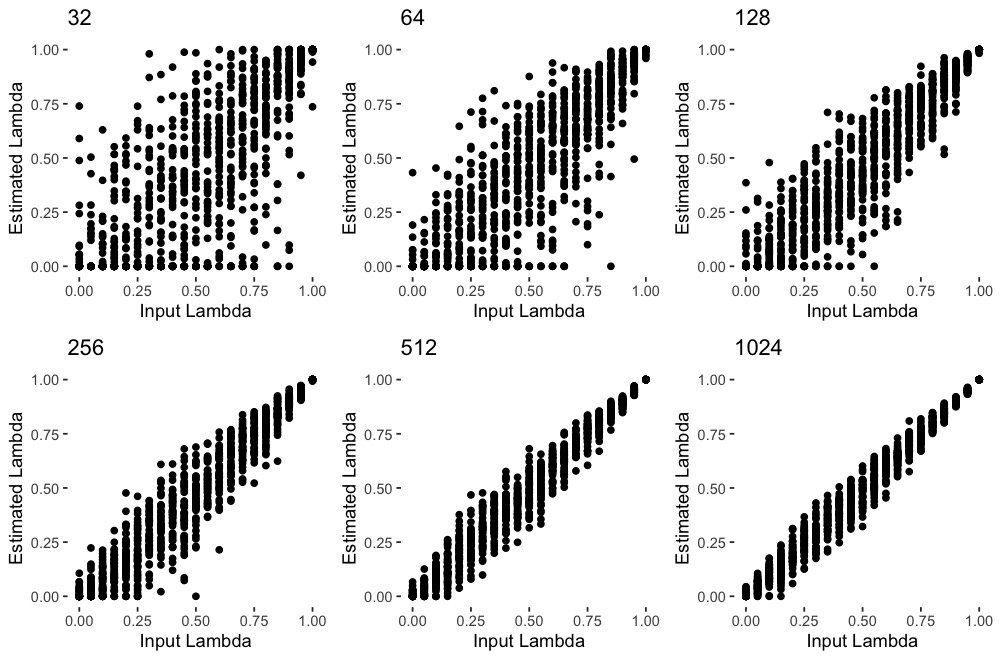
\includegraphics[width=0.95\linewidth]{Fig1}

\singlespacing \textbf{Figure 1}. Accuracy of Pagel's lambda estimations
across known lambda inputs on various tree sizes. As trees increase in
size, the estimates more closely resemble the input lambdas, however
considerable and concerning variation is apparent in trees smaller than
those with 256 tips. \hfill\break

\newpage

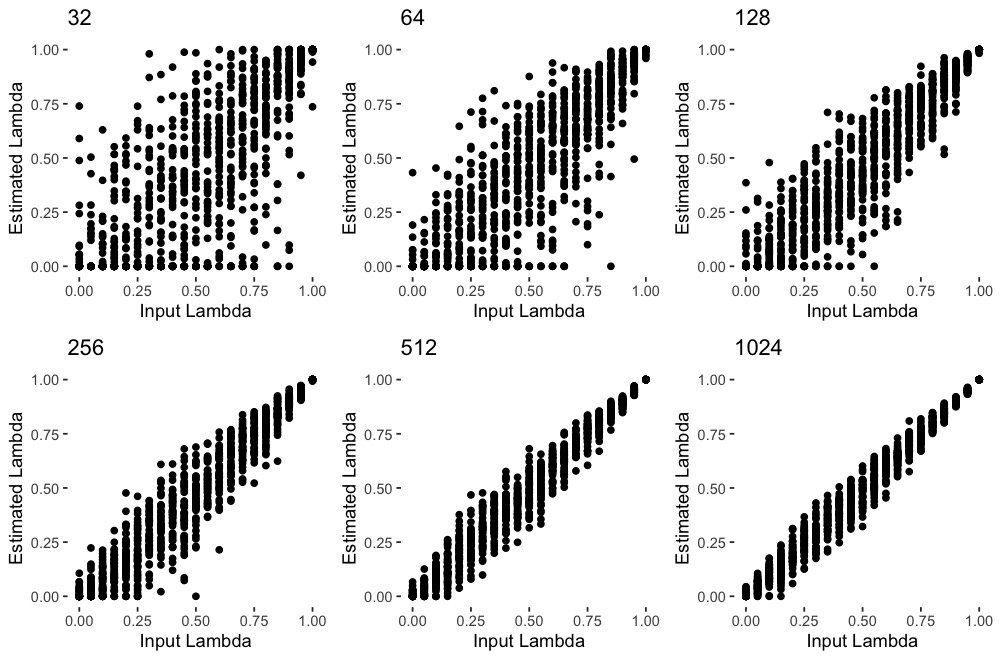
\includegraphics[width=0.95\linewidth]{Fig2}

\singlespacing \textbf{Figure 2}. Estimated ANOVA slopes under PGLS.
Across tree sizes, the mean estimated slope matches the input slope, and
as trees increase in size, the variance around this mean estimate
decreases. However, for trees with fewer than 512 tips, the error around
the estimated slope is considerable, where these analyses frequently
estimate slopes in the opposite direction of the known pattern.
\hfill\break

\newpage

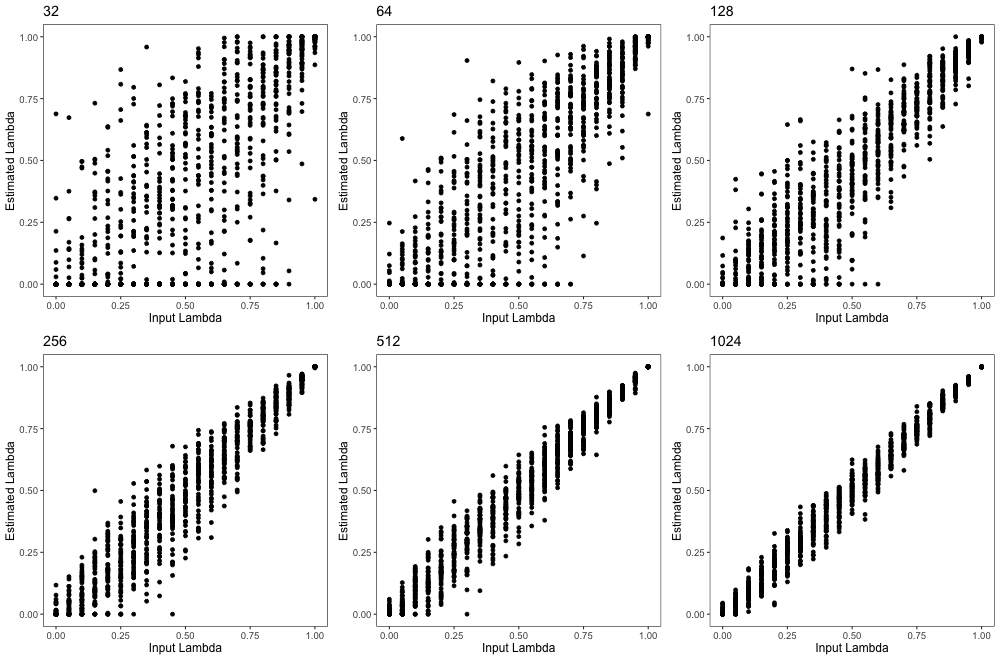
\includegraphics[width=0.95\linewidth]{Fig3}

\singlespacing \textbf{Figure 3}. Frequency of estimated lambda values
published in manuscripts in 2019. The vast majority of these values were
close to 0 or 1.

\end{document}
